\documentclass[preview]{standalone}

\usepackage{graphicx}
\usepackage{tikz}
\usepackage[format=hang]{subfig}
\usepackage{siunitx}

\newcommand{\imsize}{\linewidth}
\newlength\imagewidth
\newlength\imagescale

\begin{document}
\begin{figure}
	\subfloat[Light microscopy image, \SI{10}{x} magnification.]{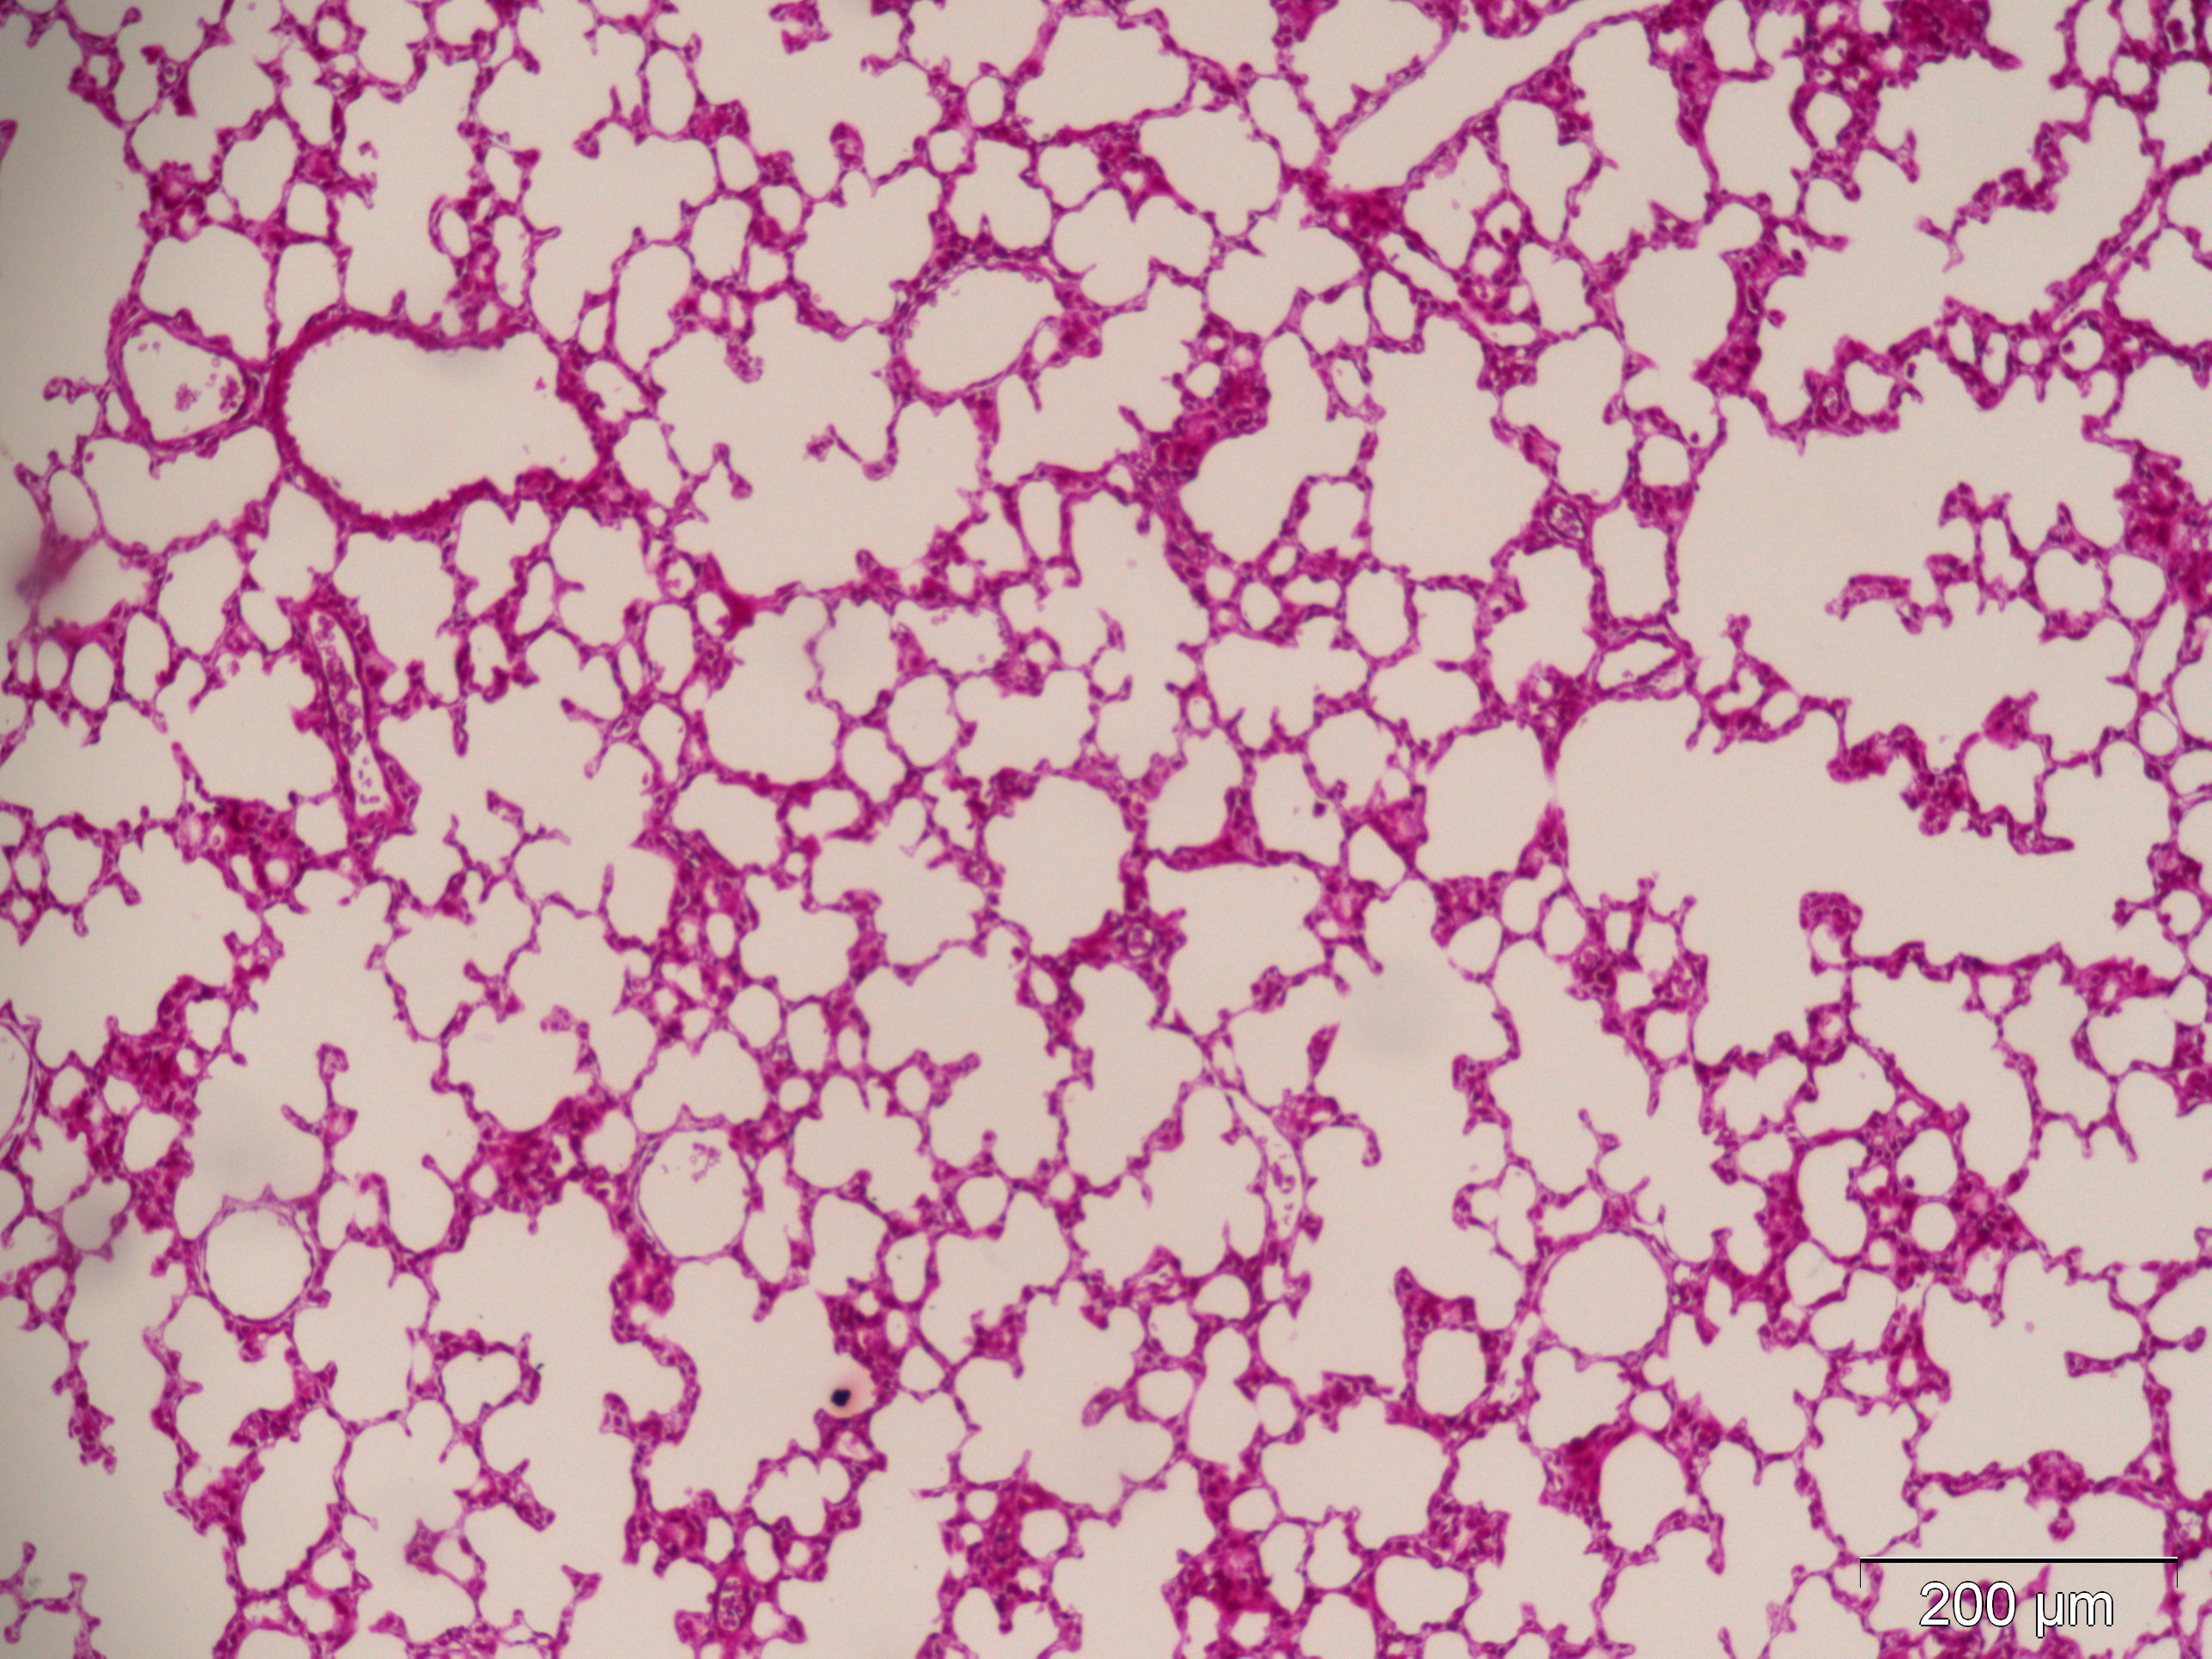
\includegraphics[width=\imsize]{../JPGs/R108C10C_I_8_1_my}}\\%
	\subfloat[Full reconstructed slice from the tomographic dataset.]{%
		\pgfmathsetlength{\imagewidth}{\imsize}%
		\pgfmathsetlength{\imagescale}{\imagewidth/2936}%
		\def\x{1814-300}% scalebar-x starting at golden ratio of image width of 2936px = 1814
		\def\y{1160}% scalebar-y at 90% of image height of 1400px = 1260
		\begin{tikzpicture}[x=\imagescale,y=-\imagescale]
			\node[anchor=north west, inner sep=0pt, outer sep=0pt] at (0,0) {\includegraphics[width=\imagewidth]{../Originals_TOMCAT/{{R108C10C_B1_mrg1024.rec.8bit.edit}}}};
			% \spy [red] on (2636,2636) in node at (0,0) [anchor=north west];
			% 2936px = 4.34528mm > 100px = 148um > 338px = 500um, 68px = 100um
			%\draw[|-|,blue,thick] (0,1468) -- (2936,1468) node [sloped,midway,above,fill=white,semitransparent,text opacity=1] {\SI{4.34528}{\milli\meter} (2936px) TEMPORARY!};
			\draw[|-|,white,thick] (\x,\y) -- (\x+338,\y) node [right] {\SI{500}{\micro\meter}};
		\end{tikzpicture}%
	}\\%
	\subfloat[Detail (middle slice) from acinus 32.
		   The segmented acinus is shown in light grey inset into the original data.
		   Scale bar is \SI{100}{\micro\meter}]{%
		\includegraphics[width=\imsize]{../Originals_TOMCAT/{{R108C10C_B1_mrg-acinus32_17_a.edit}}}%
	}%
\end{figure}%
\end{document}
